\documentclass[12pt,a4paper]{article}

\usepackage[a4paper,margin=1in]{geometry}
\usepackage{graphicx}
\usepackage{booktabs}
\usepackage{amsmath,amssymb}
\usepackage{float}
\usepackage{hyperref}
\usepackage{xcolor}
\usepackage{listings}
\usepackage{enumitem}
\usepackage{fancyhdr}
\usepackage{longtable}
\usepackage{subcaption}   % required for the 2-graphs-per-row layout
\usepackage{mathptmx}     % Times New Roman substitute font (text + math)
\usepackage{fontawesome} % for using icons

\hypersetup{colorlinks=true,linkcolor=blue,urlcolor=blue}

\pagestyle{fancy}
\fancyhf{}
\lhead{ICS1512}
\rhead{Machine Learning Algorithms Laboratory}
\cfoot{\thepage}

\lstset{
language=Python,
basicstyle=\ttfamily\small,
numbers=left,
frame=single,
breaklines=true,
showstringspaces=false
}

\begin{document}

\begin{tabular}{|p{4cm}|p{11cm}|}
\hline
Experiment No. & 1\\ \hline
Experiment Title & Working with Python Packages -- NumPy, SciPy, Scikit-Learn, Matplotlib \href{https://github.com/Poojashree81/ICS1512-Machine-Learning-Laboratory.git}{\faGithub} \\ \hline
Student Name & Poojashree V \\ \hline
Register Number & 3122247001043 \\ \hline
Faculty & Dr. Poreddy Ajay Kumar Reddy \\ \hline
Submission Date & 30th June 2026\\ \hline
\end{tabular}

\section{Objective}
To explore the functions and methods of five widely used Python libraries for machine learning—NumPy, Pandas, SciPy, Scikit-Learn, and Matplotlib—and apply them throughout a complete machine learning workflow. Five public datasets (Iris, Pima Diabetes, Loan Amount Prediction, Email Spam Classification, and Handwritten Character Recognition) were downloaded from Kaggle. For each dataset, the appropriate machine learning task (classification or regression), feature selection technique, and suitable learning algorithm were identified and validated by comparing the performance of multiple models.
 
\section{Problem Statement}
We are given five raw and unprocessed datasets which vary greatly in size, dimensionality, and modality—going from a clean numeric table with four features (Iris) to a flattened-pixel image dataset with 1024 dimensions (handwritten characters) and a 3000-dimensional bag-of-words text dataset (email spam)—and the aim is to (i) load and examine each dataset using summary statistics and visualisations, (ii) determine the correct type of machine learning task for each (that is, supervised classification or supervised regression), (iii) carry out the appropriate preprocessing for each dataset (including missing-value imputation, categorical encoding, feature scaling, and, in the case of high dimensionality, ANOVA-based feature selection), (iv) divide each dataset into training and test parts, (v) train a representative set of Scikit-Learn algorithms on each dataset, and (vi) assess and compare their performance using metrics appropriate to the task. The result of the experiment is a task-identification table for all five datasets together with quantitative performance benchmarks for each of the algorithms tested.
 
\section{ML Task Identification}
 
\begingroup
\small
\begin{longtable}{|p{2.7cm}|p{2.3cm}|p{3.6cm}|p{3.9cm}|}
\hline
\textbf{Dataset} & \textbf{Type of ML Task} & \textbf{Feature Selection Technique} & \textbf{Suitable ML Algorithm (empirically best)} \\
\hline
\endhead
Iris Dataset & Supervised, multi-class classification (3 classes) & Not required -- only 4 low-noise, highly discriminative features & SVM (linear kernel) -- 100\% test accuracy \\
\hline
Loan Amount Prediction & Supervised regression (continuous target) & Not applied -- only 5 numeric predictors survive cleaning; all retained & Gradient Boosting Regressor -- best (still weak) R\textsuperscript{2} = 0.214 \\
\hline
Predicting Diabetes & Supervised, binary classification & Not applied -- all 8 clinical features are domain-relevant & Gradient Boosting / Random Forest -- $\approx$75\% accuracy \\
\hline
Classification of Email Spam & Supervised, binary classification, high-dimensional bag-of-words & SelectKBest (ANOVA F-test), top 300 of 3000 word-count features & Random Forest -- 96.04\% accuracy, ROC-AUC 0.993 \\
\hline
Handwritten Character Recognition (62-class, used as the MNIST-style task) & Supervised, multi-class classification, high-dimensional raw pixels & SelectKBest (ANOVA F-test), top 100 of 1024 pixel features & Random Forest -- 35.19\% accuracy (best of the classical models tried; a CNN is recommended for production use) \\
\hline
\end{longtable}
\endgroup
 
\section{Dataset Description}
\begingroup
\small
\begin{longtable}{|p{2.6cm}|p{2.6cm}|p{1.3cm}|p{1.3cm}|p{1.9cm}|p{1.7cm}|p{1.7cm}|}
\hline
\textbf{Dataset} & \textbf{Source} & \textbf{Samples} & \textbf{Features} & \textbf{Classes / Target} & \textbf{Missing Values} & \textbf{Train-Test Split} \\
\hline
\endhead
Iris & Kaggle -- Iris Species dataset & 150 & 4 (numeric) & 3 (Species) & None & 80\% / 20\% (stratified) \\
\hline
Diabetes & Kaggle -- Pima Indians Diabetes Database & 768 & 8 (numeric) & 2 (Outcome) & None & 80\% / 20\% (stratified) \\
\hline
Loan Amount & Kaggle -- Loan Prediction dataset (\texttt{train\_u6lujuX\_CVtuZ9i.csv}) & 592\footnote{614 rows in the raw file; reduced to 592 after dropping rows with a missing \texttt{LoanAmount} target.} & 11 (mixed) & Continuous (LoanAmount, in thousands) & Yes -- up to 8.28\% in \texttt{Credit\_History} & 80\% / 20\% \\
\hline
Email Spam & Kaggle -- Email Spam Classification (word-count) dataset & 5172 & 3000 (word counts) & 2 (Prediction: spam/ham) & None & 80\% / 20\% (stratified) \\
\hline
Handwritten Characters & Kaggle -- Handwritten Character Recognition (English) dataset & 3410 & 1024 (32$\times$32 grayscale pixels, flattened) & 62 (0--9, A--Z, a--z) & None & 80\% / 20\% (stratified) \\
\hline
\end{longtable}
\endgroup
 
\section{Exploratory Data Analysis}
A single reusable \texttt{perform\_eda()} routine was written to compute shape, dtypes, sum-
mary statistics, missing-value counts, IQR- and Z-score-based outlier counts, and to
Generate boxplots, plots of the distribution, correlation plots, and plots of the target distribution. For the two high-
dimensional datasets (Email Spam with 3000 features, Handwritten Characters with 1024
features) the function was designed to automatically skip the per-feature histogram/box-
plot/correlation plots once feature count exceeds 30, since 3000 individual histograms
would be unreadable and computationally wasteful – only the target-class distribution is
plotted for those two.
 
\subsection{Iris Dataset}
\begin{figure}[H]
\centering
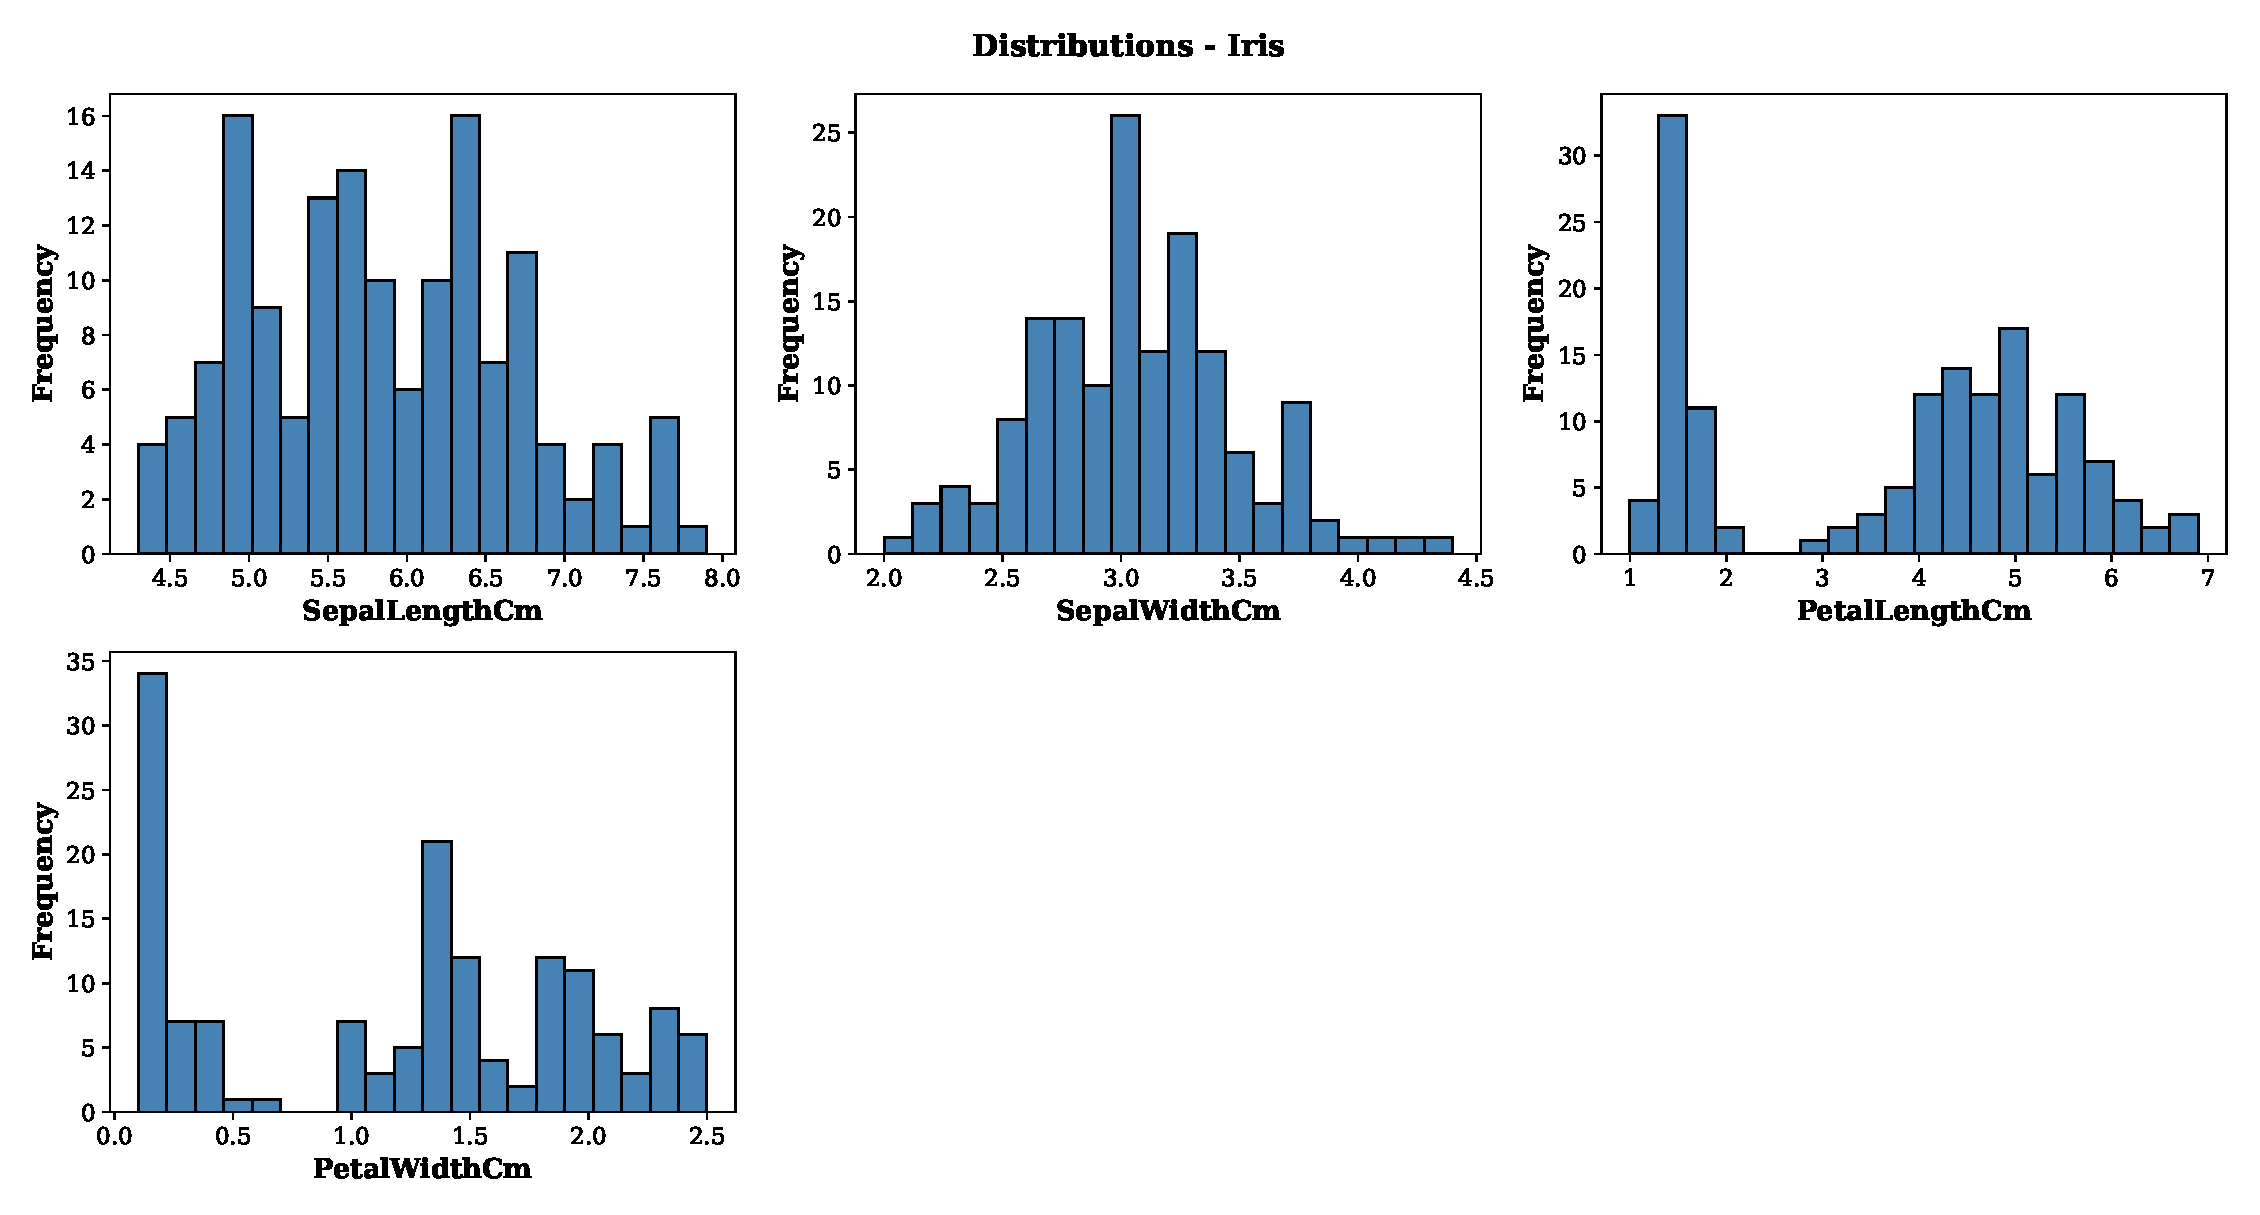
\includegraphics[width=0.7\linewidth]{figures/Iris_histograms.eps}
\caption{Feature-wise histograms of the Iris dataset (one-column layout, all 4 numeric features).}
\label{fig:iris_hist}
\end{figure}
\textbf{Inference:} Looking at Figure~\ref{fig:iris_hist}, all four features come out unimodal or bimodal, and there's no missing data to worry about here. Petal length and petal width stand out in particular -- both show a clear bimodal/trimodal spread, which hints that these two features are doing most of the work separating the three species. The sepal measurements aren't nearly as clean; they overlap quite a bit between \textit{Iris-versicolor} and \textit{Iris-virginica}. This lines up with what's usually reported about this dataset elsewhere, where petal measurements tend to be the stronger predictors. Sepal width, on the other hand, comes out the most symmetric and closest to a normal distribution of the four.
 
\begin{figure}[H]
\centering
\begin{subfigure}[b]{0.48\linewidth}
\centering
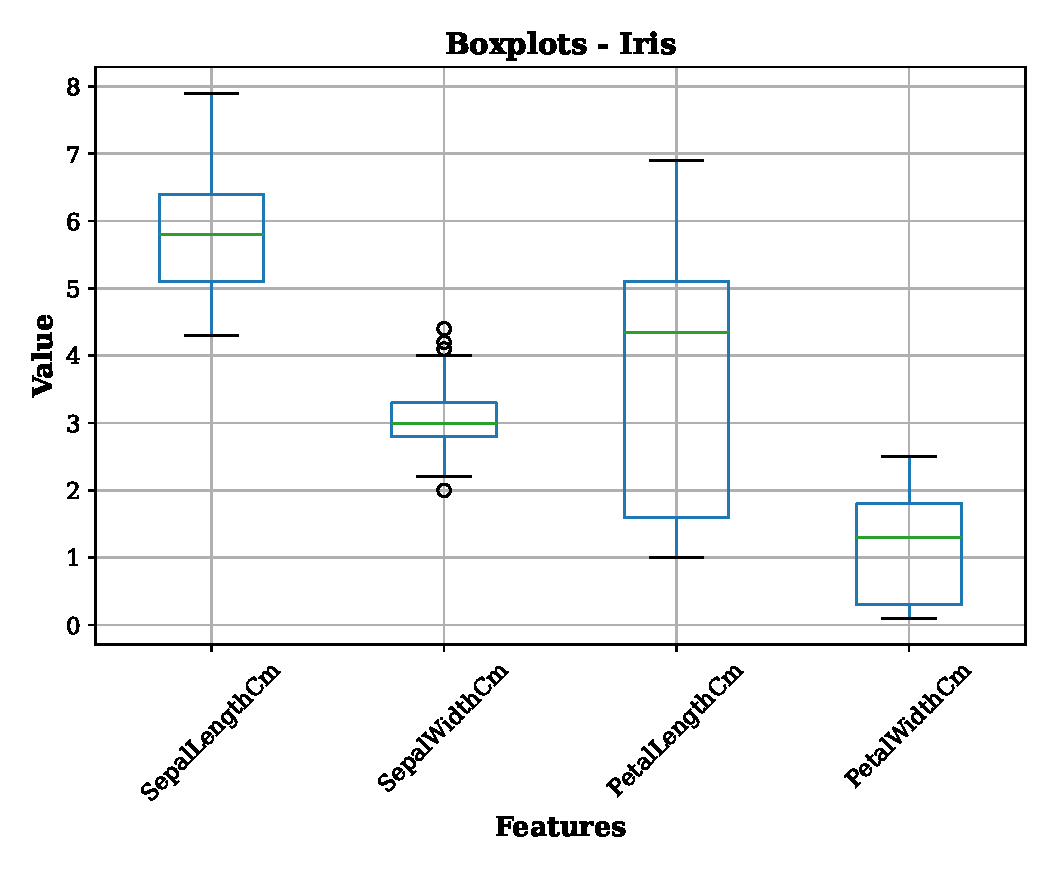
\includegraphics[width=\linewidth]{figures/Iris_boxplots.eps}
\caption{Boxplots of the 4 Iris features.}
\end{subfigure}
\hfill
\begin{subfigure}[b]{0.48\linewidth}
\centering
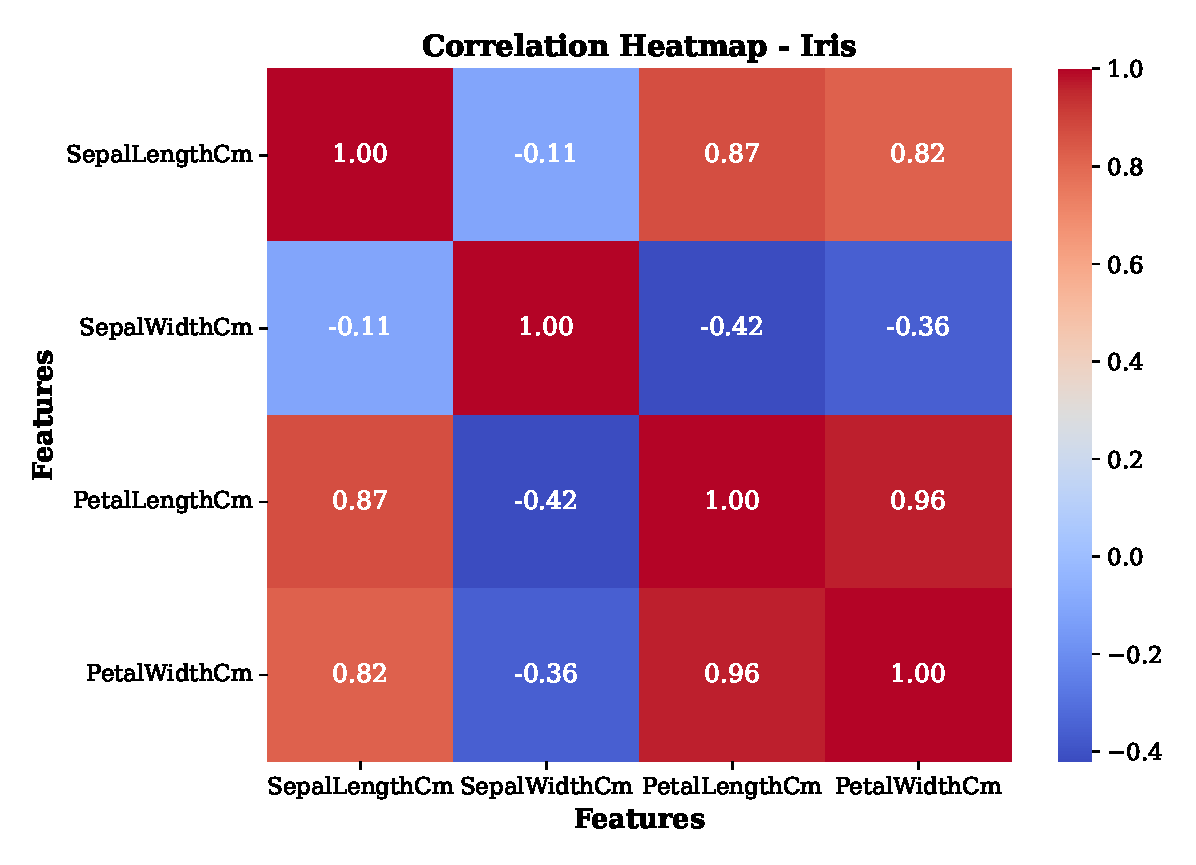
\includegraphics[width=\linewidth]{figures/Iris_correlation_heatmap.eps}
\caption{Correlation heatmap of the 4 Iris features.}
\end{subfigure}
\caption{Iris dataset -- spread and correlation diagnostics (two-column layout).}
\label{fig:iris_box_corr}
\end{figure}
\textbf{Inference:} Only \texttt{SepalWidthCm} shows any real outliers -- 4 by the IQR rule, just 1 under the stricter $|z|>3$ cutoff -- and the other three features have none at all, so this dataset is about as clean as they come. The correlation heatmap in Figure~\ref{fig:iris_box_corr} tells an interesting story: petal length and petal width are almost perfectly correlated ($r \approx 0.96$), and both also track sepal length fairly closely ($r \approx 0.87$ and $0.82$ respectively). Sepal width barely correlates with anything, if anything slightly negatively. That petal length/petal width redundancy is probably why a plain linear boundary already separates the classes almost perfectly.
 
\begin{figure}[H]
\centering
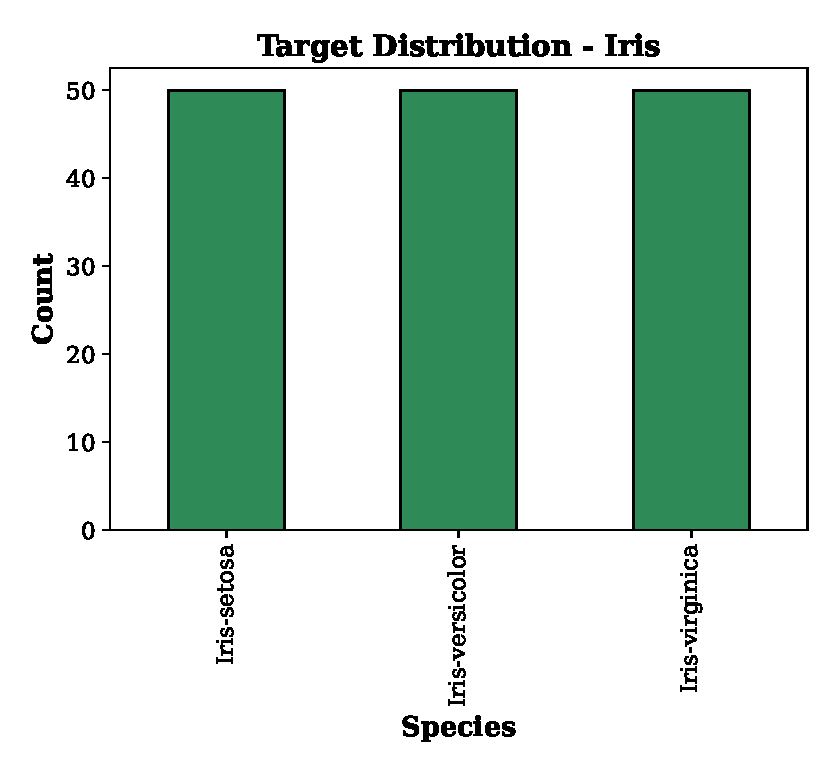
\includegraphics[width=0.55\linewidth]{figures/Iris_target_distribution.eps}
\caption{Class distribution of the target variable \texttt{Species}.}
\label{fig:iris_target}
\end{figure}
\textbf{Inference:} Each class has exactly 50 samples, so the target is perfectly balanced. That means no oversampling or class-weighting is needed -- accuracy alone is a fair metric to optimize for.
 
\subsection{Diabetes Dataset}
\begin{figure}[H]
\centering
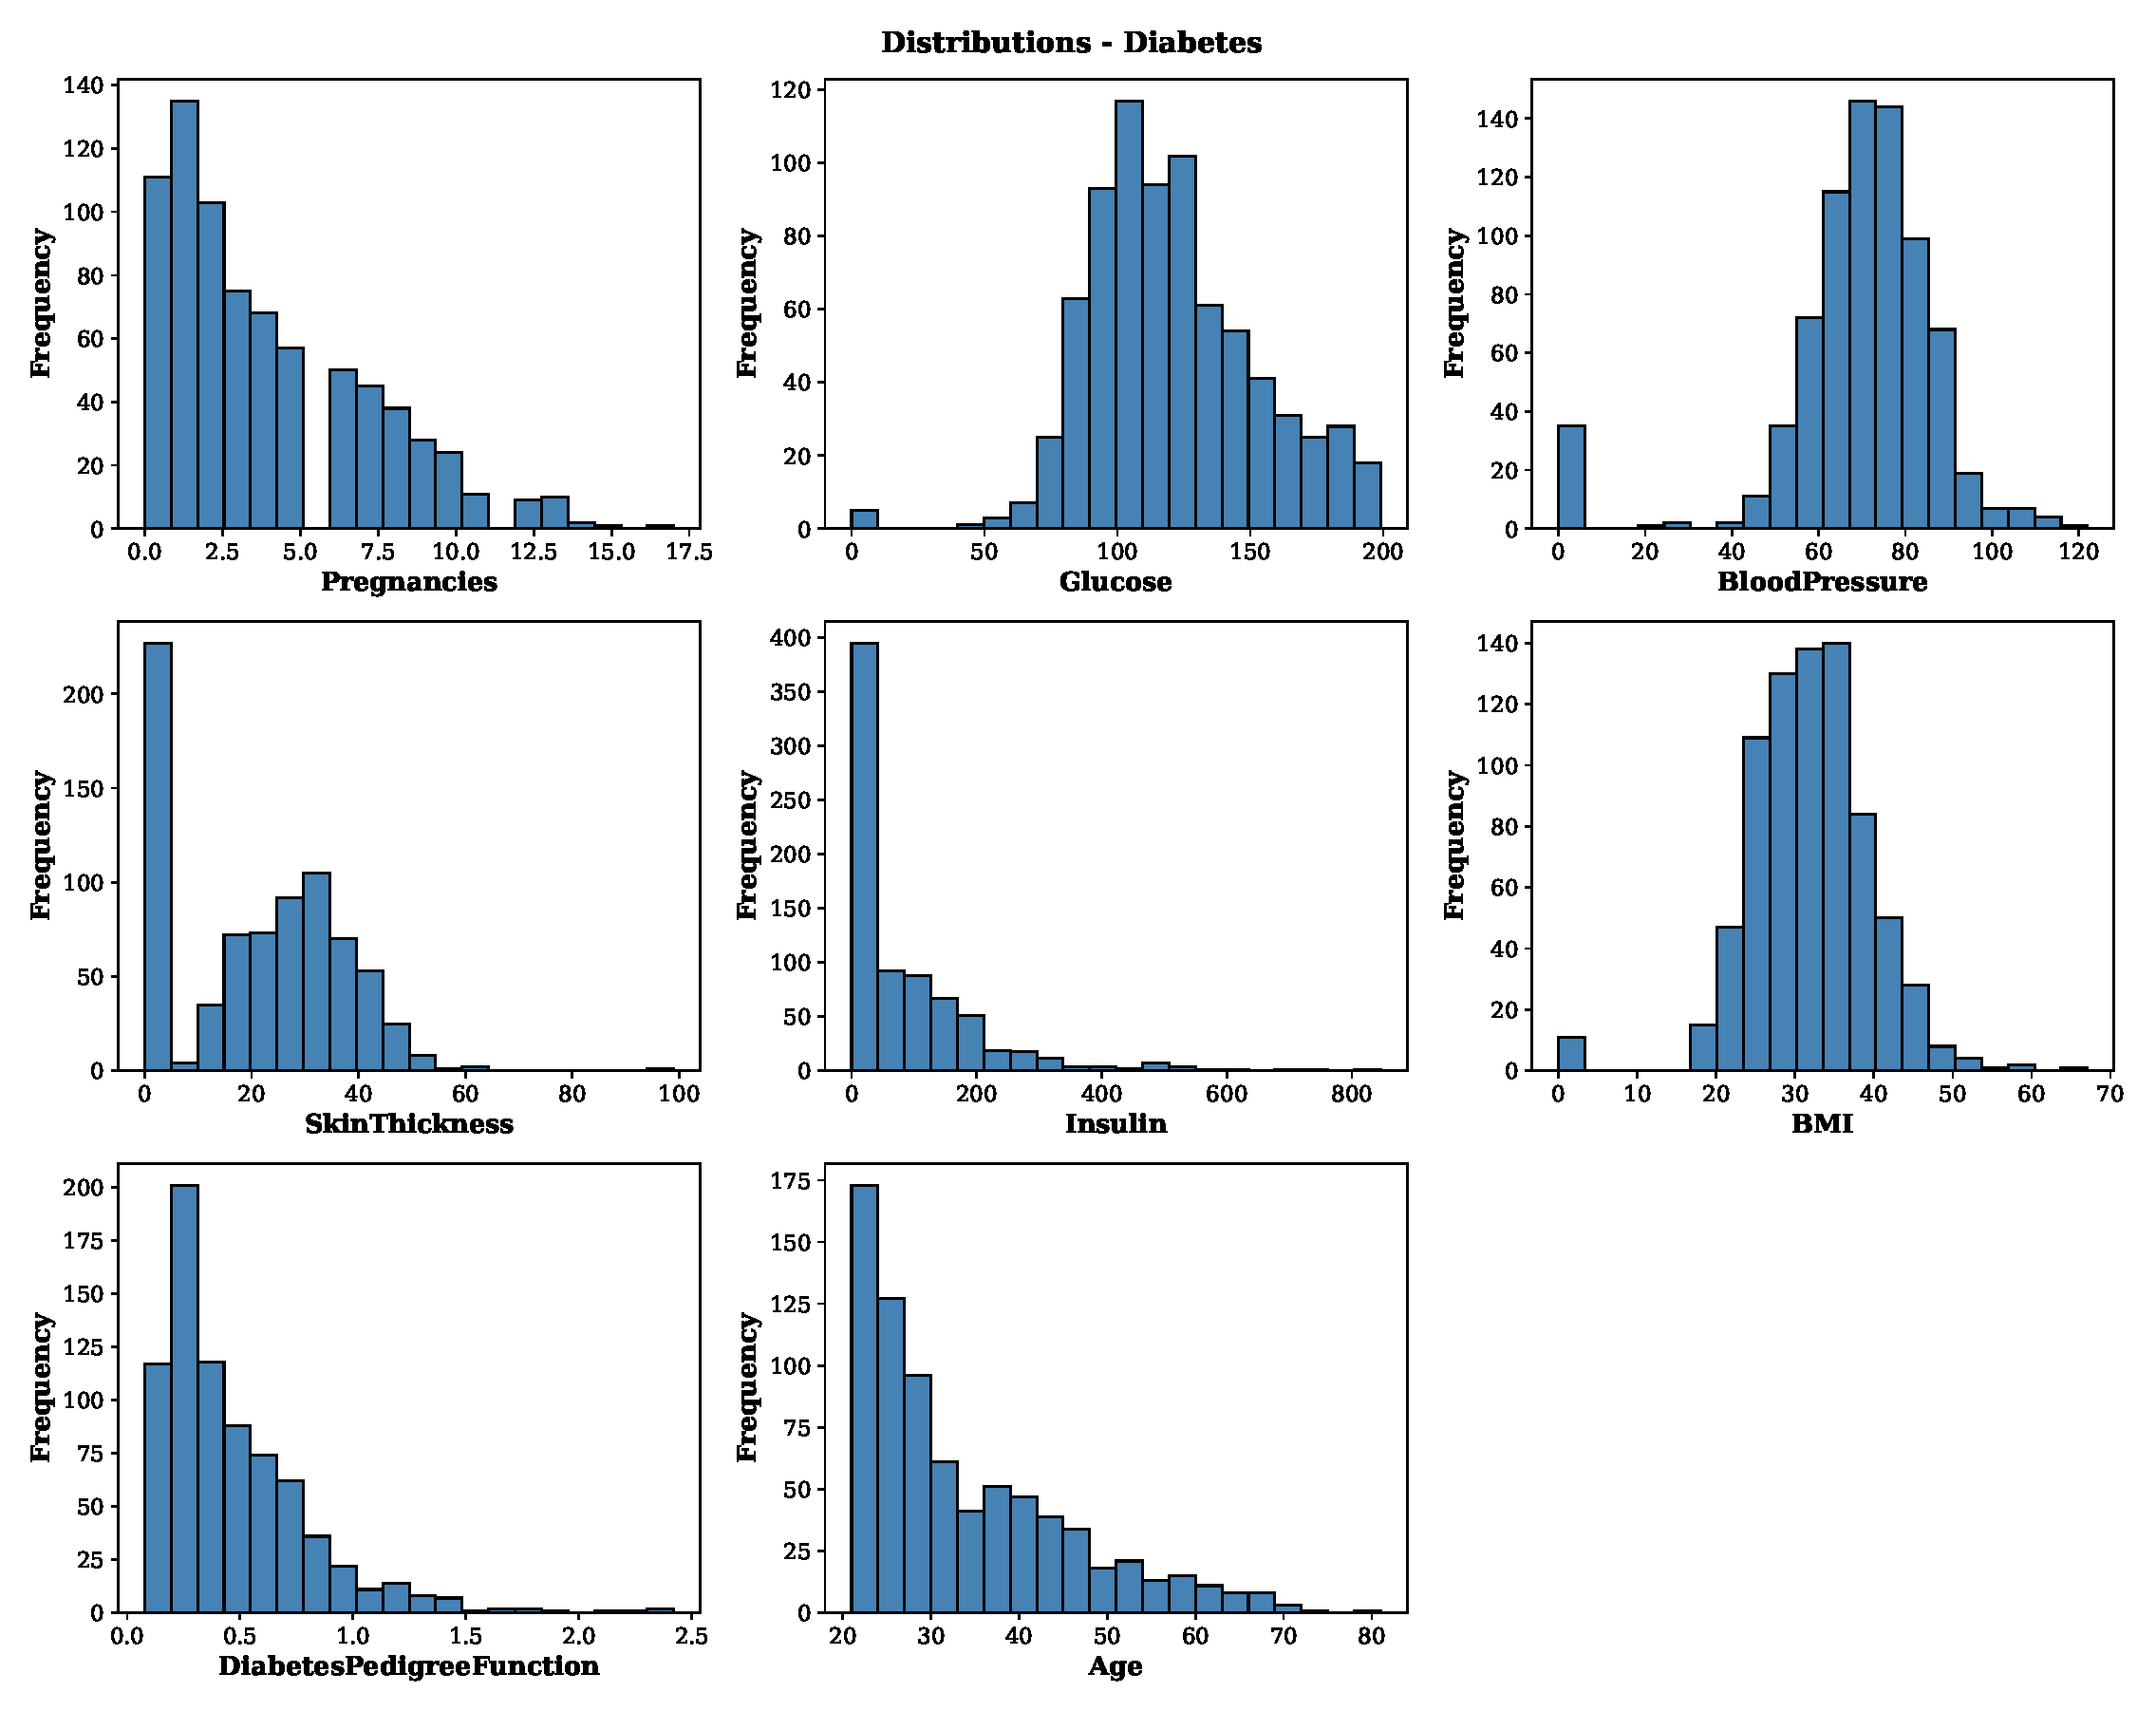
\includegraphics[width=0.95\linewidth]{figures/Diabetes_histograms.eps}
\caption{Feature-wise histograms of the Pima Diabetes dataset (one-column layout, all 8 numeric features).}
\label{fig:diab_hist}
\end{figure}
\textbf{Inference:} \texttt{Insulin} and \texttt{DiabetesPedigreeFunction} are both heavily right-skewed with long tails. \texttt{Glucose}, \texttt{BloodPressure}, and \texttt{BMI} look closer to normal at a glance, but each one has a suspicious spike at exactly zero. That's not physiologically possible -- a living patient can't have zero blood pressure or zero BMI -- so these are almost certainly missing values that got encoded as zero rather than true readings. \texttt{Age} is right-skewed as well, which just reflects a younger-skewing cohort overall. This zero-inflation is likely the main reason the IQR/Z-score outlier counts come out so high for several of these columns.
 
\begin{figure}[H]
\centering
\begin{subfigure}[b]{0.48\linewidth}
\centering
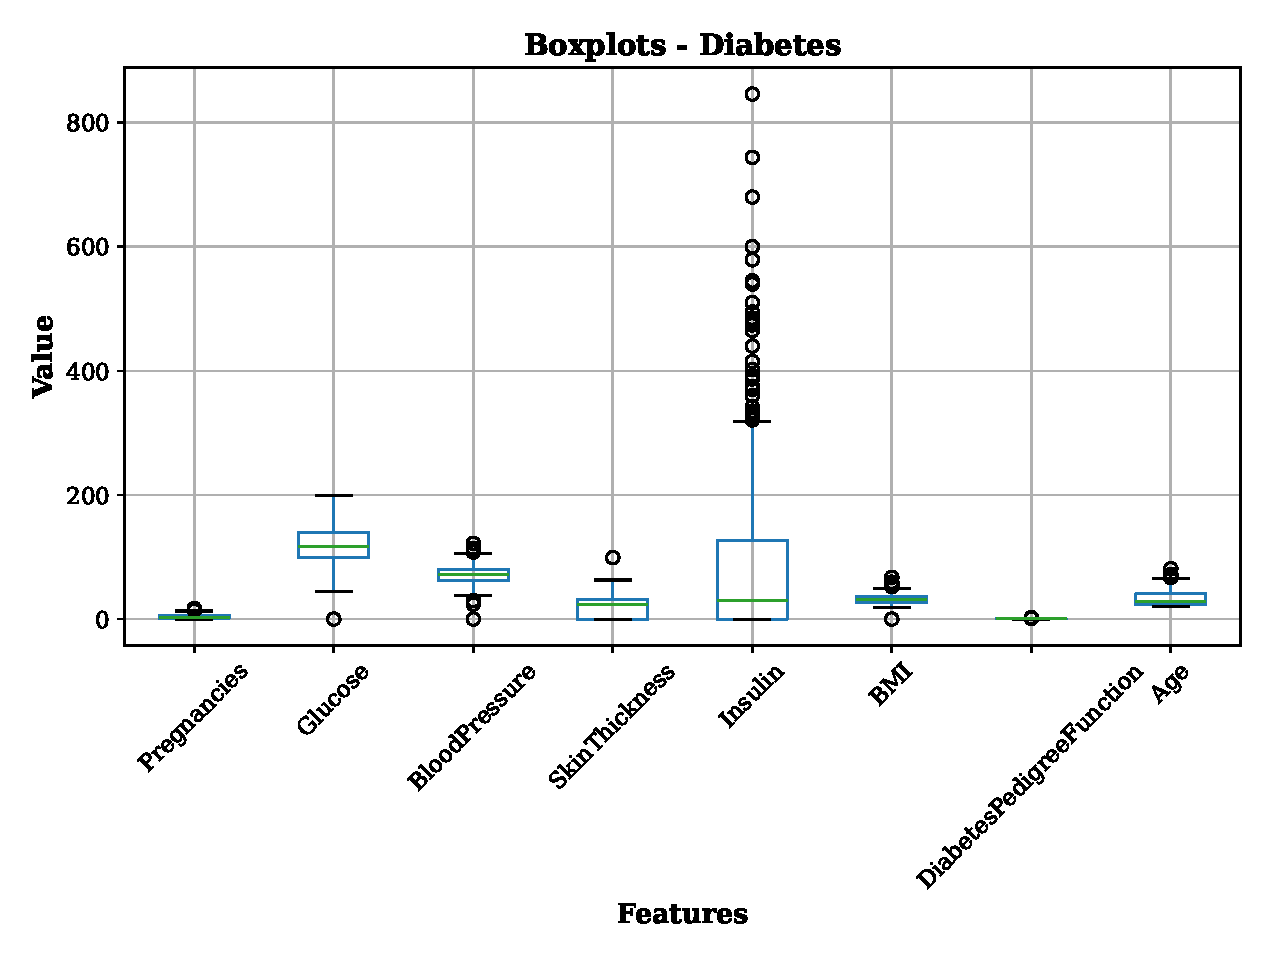
\includegraphics[width=\linewidth]{figures/Diabetes_boxplots.eps}
\caption{Boxplots of the 8 Diabetes features.}
\end{subfigure}
\hfill
\begin{subfigure}[b]{0.48\linewidth}
\centering
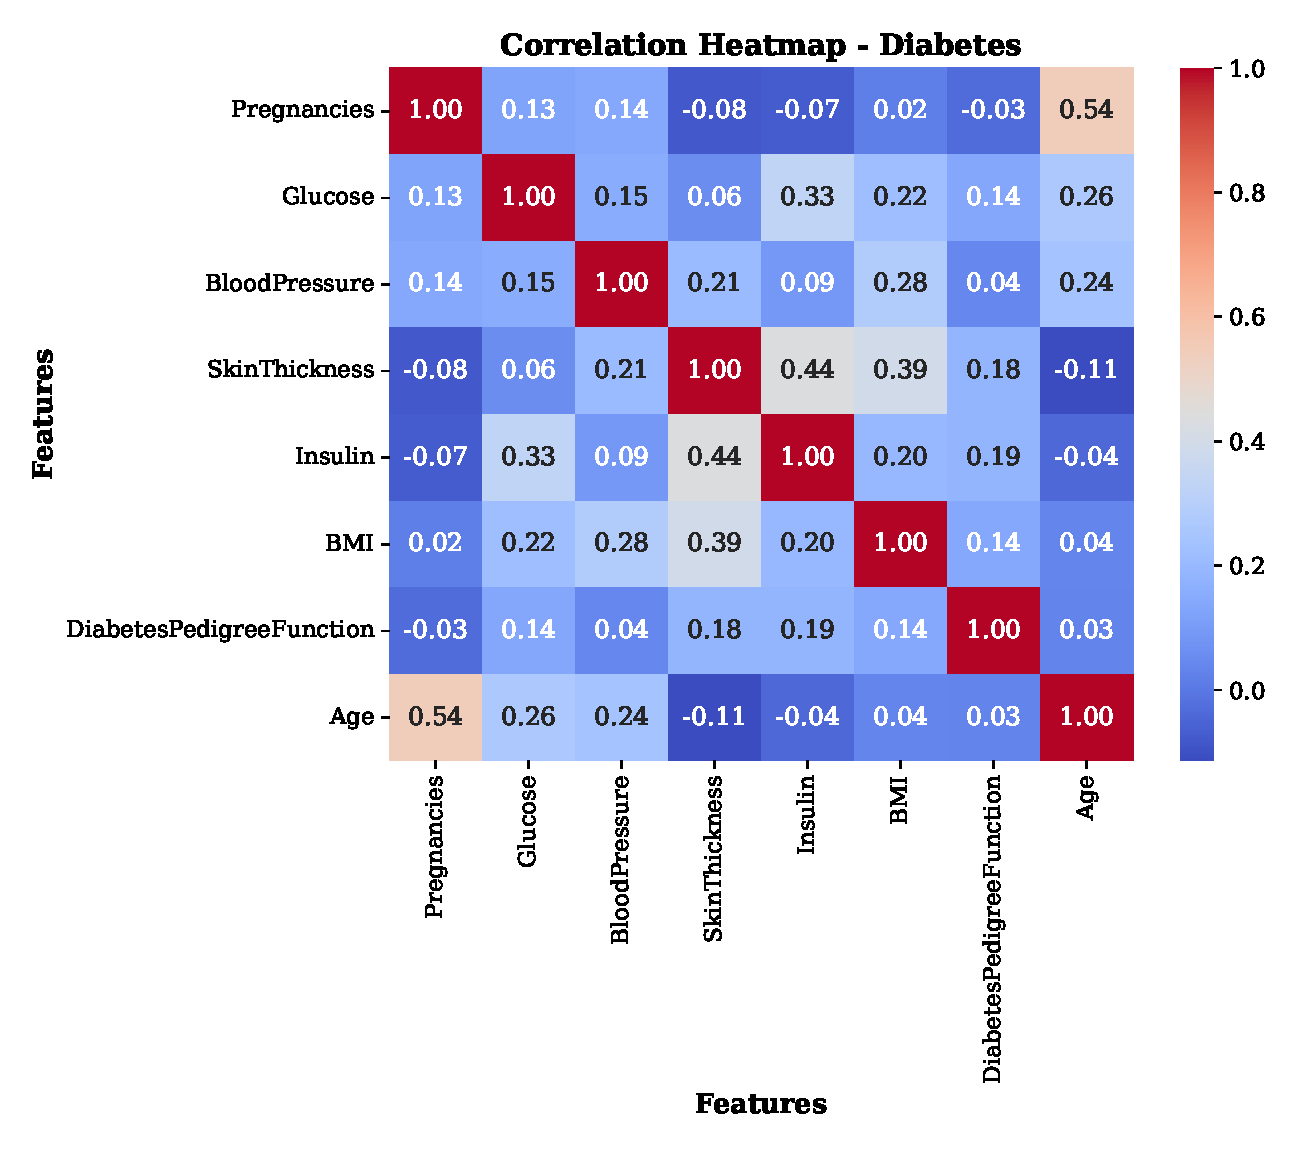
\includegraphics[width=\linewidth]{figures/Diabetes_correlation_heatmap.eps}
\caption{Correlation heatmap of the 8 Diabetes features.}
\end{subfigure}
\caption{Diabetes dataset -- spread and correlation diagnostics (two-column layout).}
\label{fig:diab_box_corr}
\end{figure}
\textbf{Inference:} \texttt{BloodPressure} has the most outliers of any column (45 by IQR, 35 by Z-score), which again traces back to those disguised zero readings. \texttt{Insulin} comes next with 34 IQR outliers, matching how skewed its distribution already looked in Figure~\ref{fig:diab_hist}. From the heatmap, \texttt{Glucose} correlates most strongly with the target \texttt{Outcome} -- which lines up with clinical intuition, since elevated blood glucose is the primary diabetes marker. \texttt{Age} and \texttt{Pregnancies} are moderately correlated with each other too, which isn't surprising biologically. Nothing here looks severely collinear, so multicollinearity wasn't a real concern for the linear models tested.
 
\begin{figure}[H]
\centering
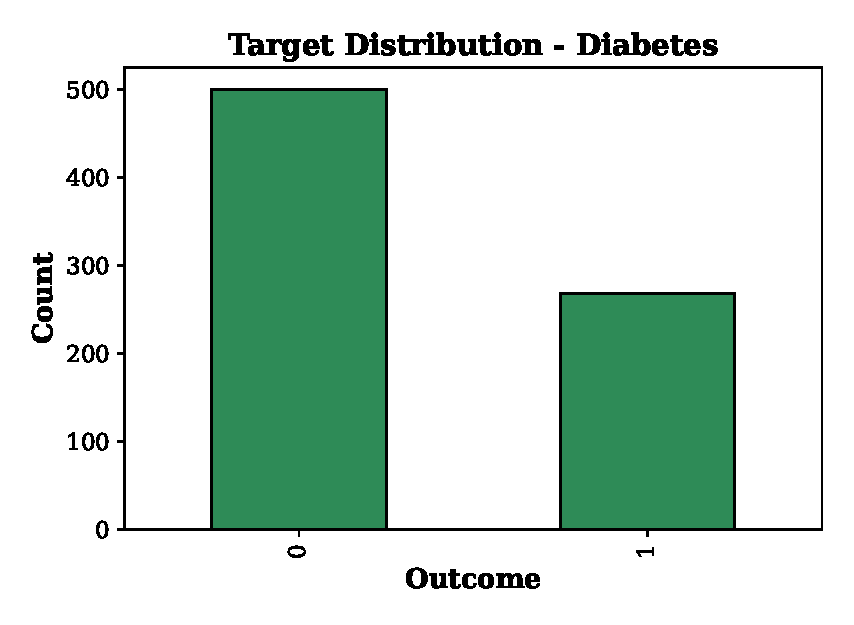
\includegraphics[width=0.55\linewidth]{figures/Diabetes_target_distribution.eps}
\caption{Class distribution of the target variable \texttt{Outcome}.}
\label{fig:diab_target}
\end{figure}
\textbf{Inference:} There's a class imbalance here -- roughly 65\% non-diabetic (Outcome = 0) versus 35\% diabetic (Outcome = 1), which matches the 0.349 mean reported for \texttt{Outcome} in the summary statistics. Because of that imbalance, we tracked \texttt{Precision}, \texttt{Recall}, and \texttt{F1} (weighted average) alongside raw accuracy in the results rather than relying on accuracy on its own.
 
\subsection{Loan Amount Prediction Dataset}
\begin{figure}[H]
\centering
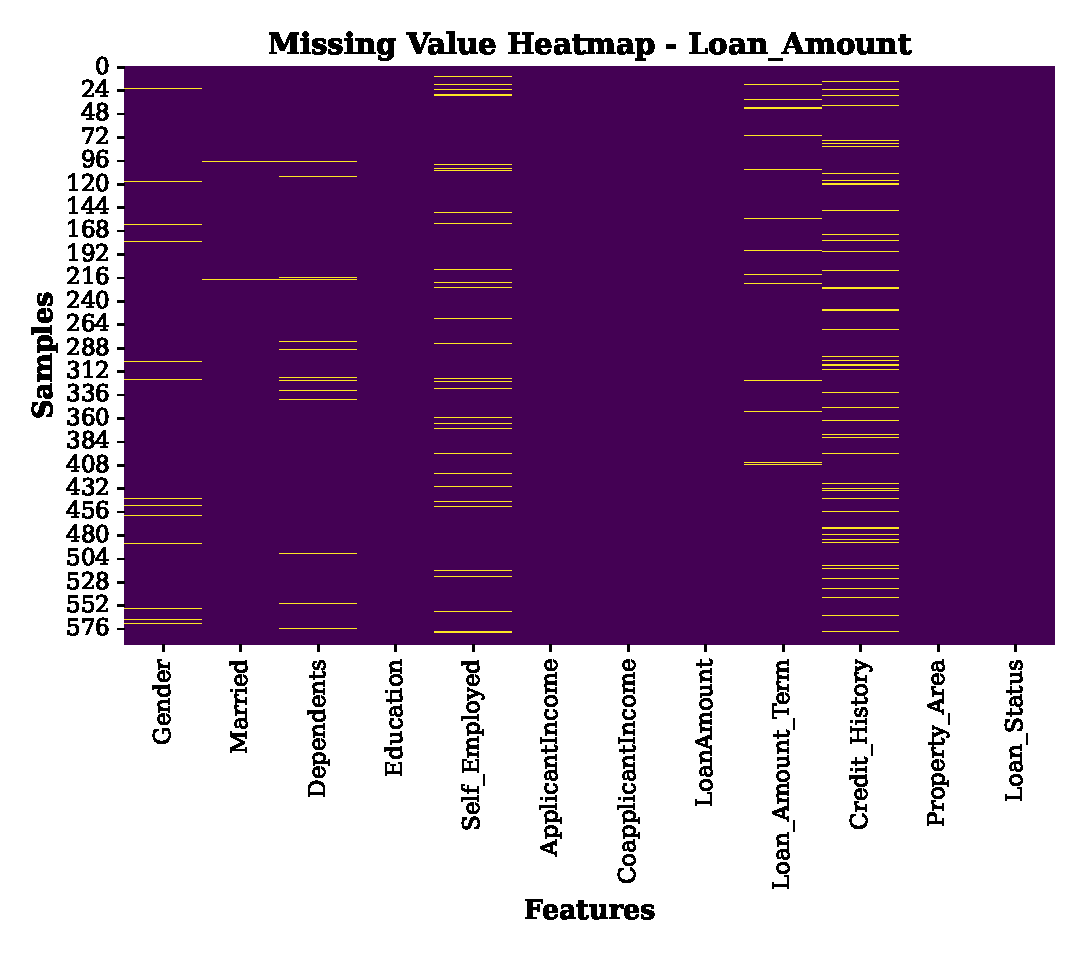
\includegraphics[width=0.85\linewidth]{figures/Loan_Amount_missing_heatmap.eps}
\caption{Missing-value heatmap of the Loan Amount dataset (yellow = missing).}
\label{fig:loan_missing}
\end{figure}
\textbf{Inference:} This is the one dataset, out of the five, that genuinely has missing values. \texttt{Credit\_History} has the most gaps at 8.28\%, followed by \texttt{Self\_Employed} (5.24\%), \texttt{Loan\_Amount\_Term} (2.36\%), \texttt{Gender} and \texttt{Dependents} (around 2.2\% each), and \texttt{Married} (just 0.34\%). The missingness doesn't cluster in any particular row or block -- it looks more like applicants simply skipping optional fields here and there than any systematic problem with data collection.
 
\begin{figure}[H]
\centering
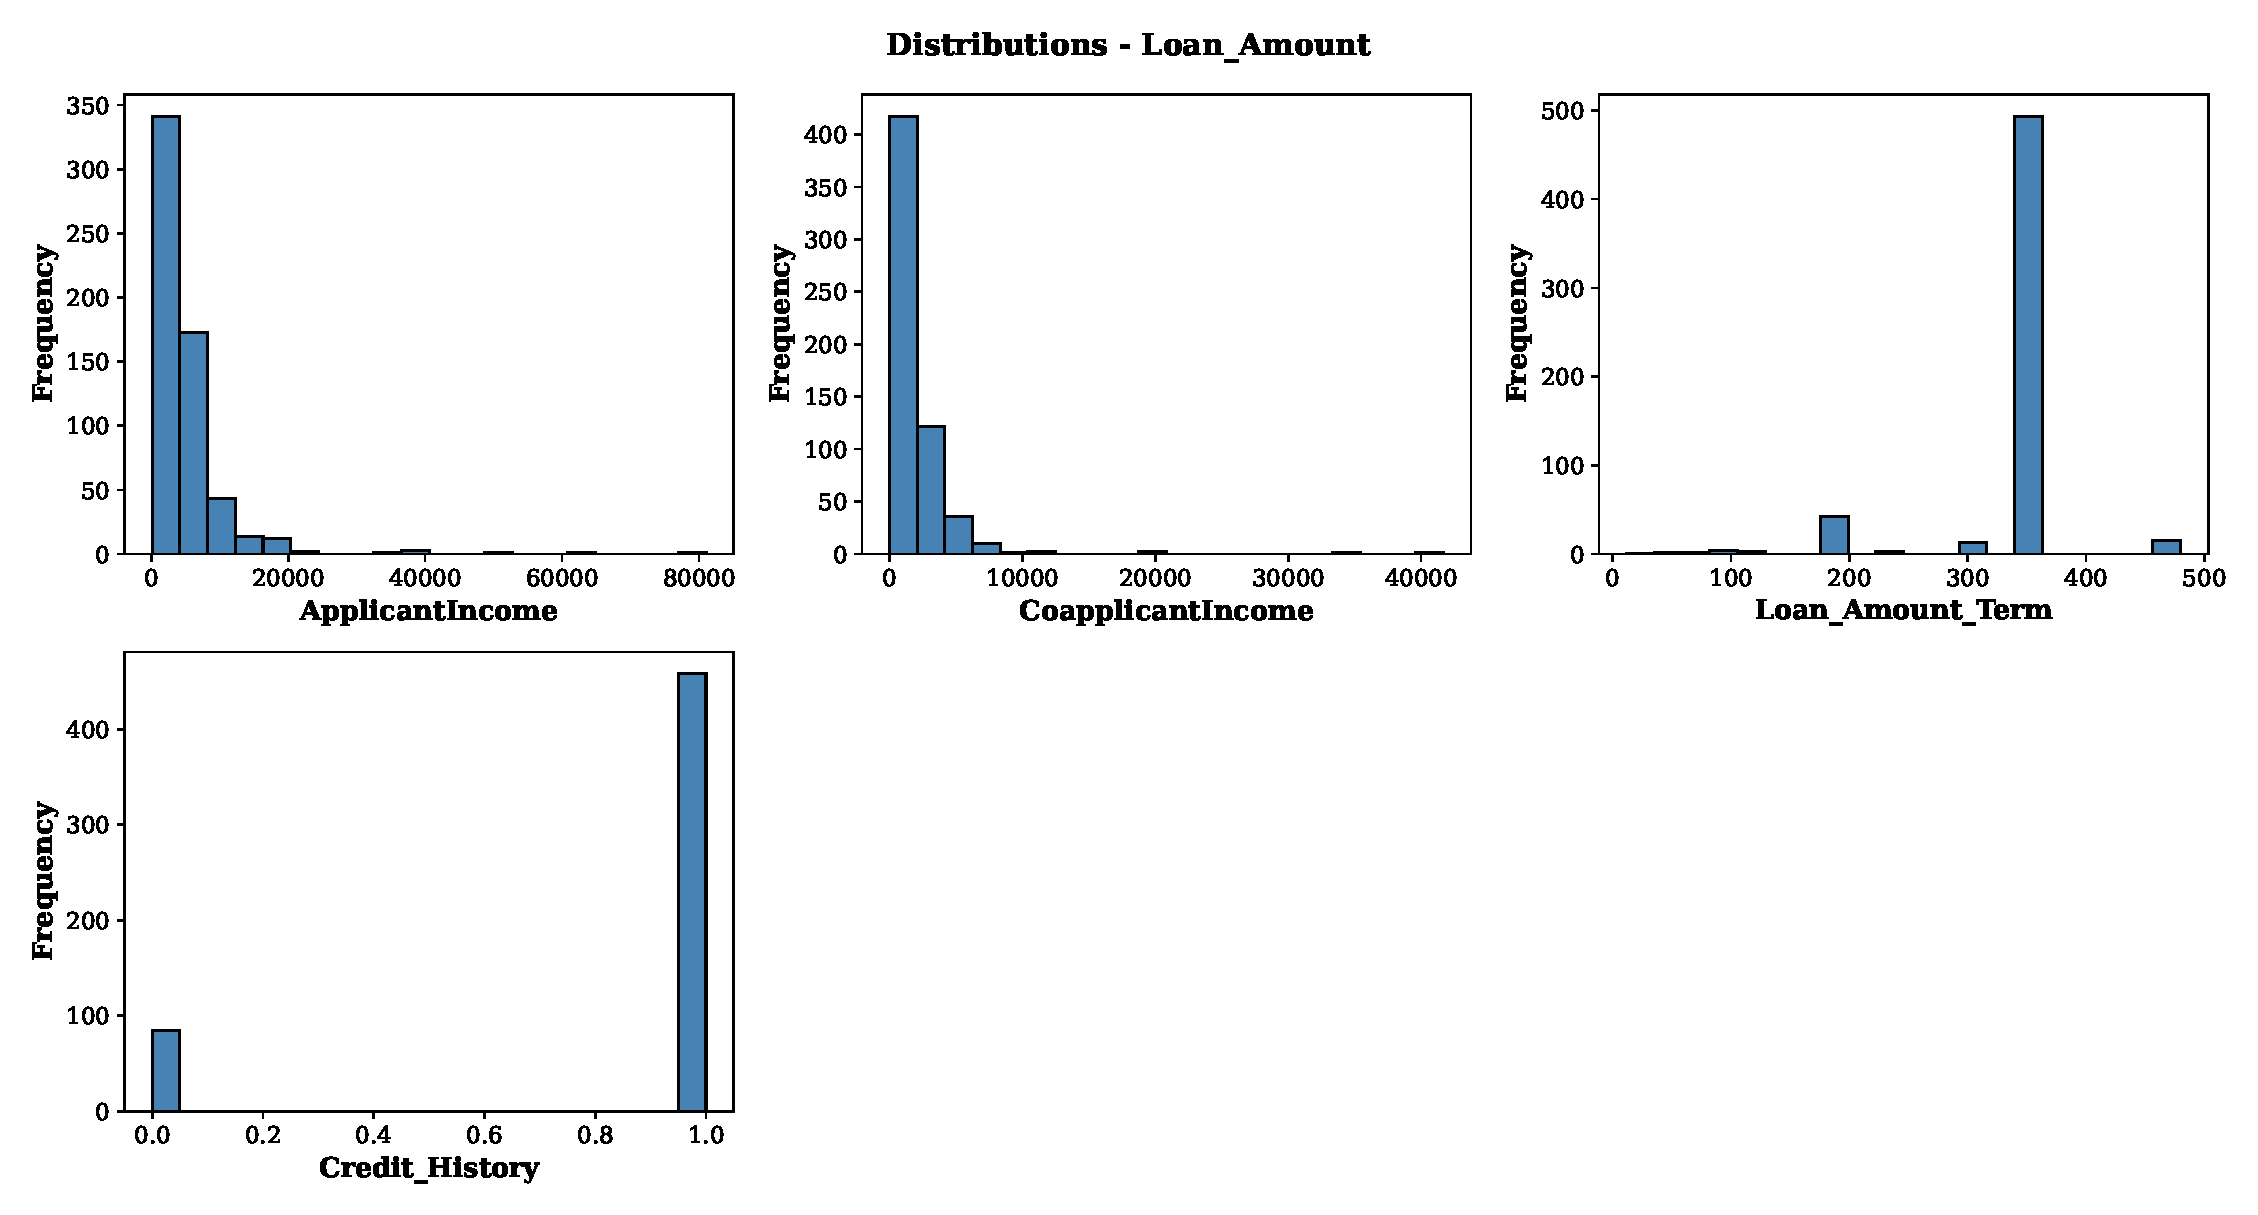
\includegraphics[width=0.95\linewidth]{figures/Loan_Amount_histograms.eps}
\caption{Feature-wise histograms of the Loan Amount dataset (one-column layout).}
\label{fig:loan_hist}
\end{figure}
\textbf{Inference:} \texttt{ApplicantIncome} and \texttt{CoapplicantIncome} are both extremely right-skewed -- a small number of very high earners stretch the axis out, and that's essentially why we get 49 and 18 IQR outliers for these two columns. \texttt{Loan\_Amount\_Term} is almost entirely a single spike at 360 months (the standard 30-year tenure), with just a few short-tenure cases pulling away from it. \texttt{Credit\_History} is essentially binary (0/1) rather than continuous, so it's not too surprising it also got flagged with 85 ``outliers'' by the IQR rule -- that's really just an artifact of running IQR on a near-binary column, not a genuine anomaly.
 
\begin{figure}[H]
\centering
\begin{subfigure}[b]{0.48\linewidth}
\centering
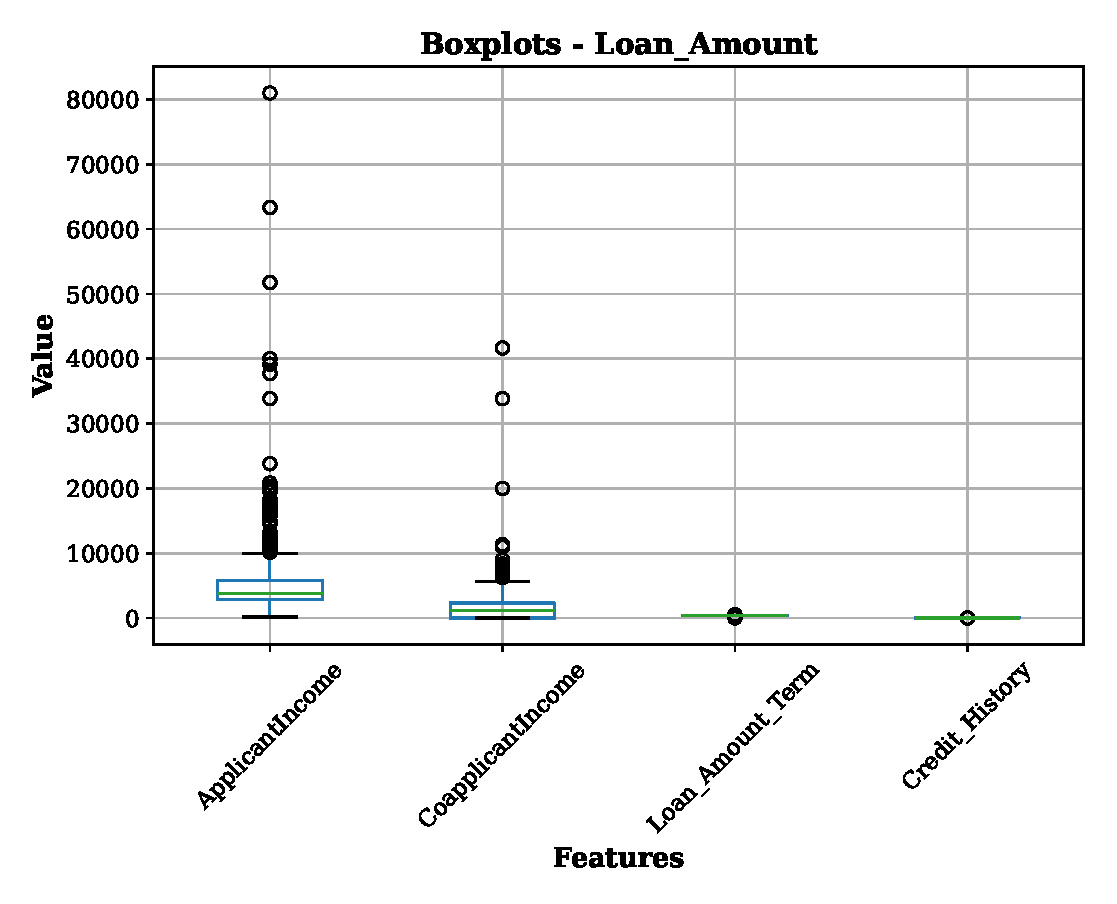
\includegraphics[width=\linewidth]{figures/Loan_Amount_boxplots.eps}
\caption{Boxplots of the Loan Amount numeric features.}
\end{subfigure}
\hfill
\begin{subfigure}[b]{0.48\linewidth}
\centering
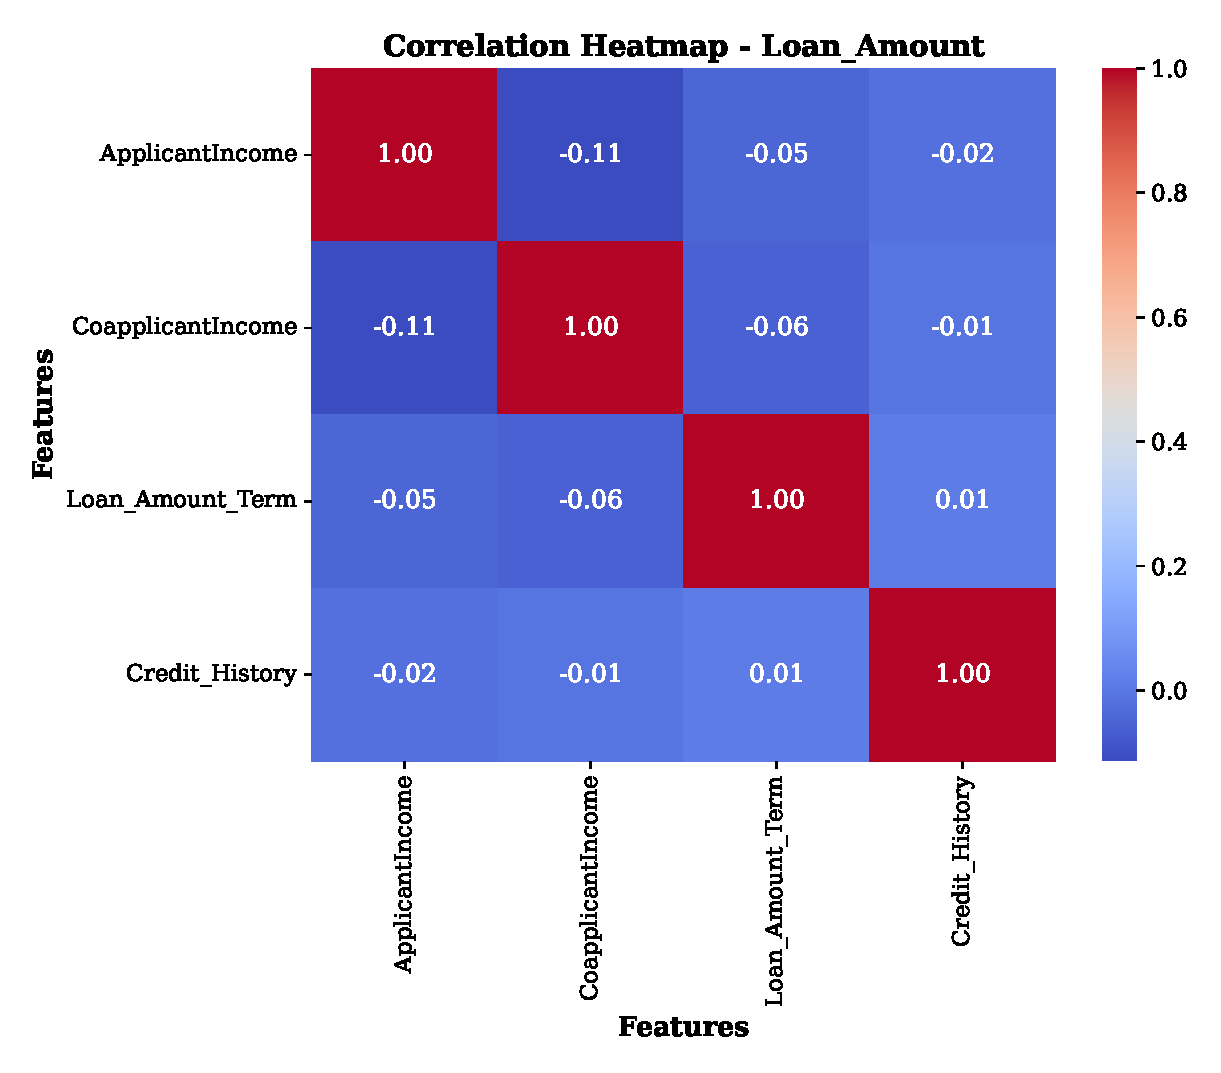
\includegraphics[width=\linewidth]{figures/Loan_Amount_correlation_heatmap.eps}
\caption{Correlation heatmap of the Loan Amount numeric features.}
\end{subfigure}
\caption{Loan Amount dataset -- spread and correlation diagnostics (two-column layout).}
\label{fig:loan_box_corr}
\end{figure}
\textbf{Inference:} The boxplots make the income-related outliers pretty obvious once everything is plotted on a shared axis -- they dwarf the rest of the distribution. \texttt{Credit\_History} shows up as a thin bar near 1, since roughly 84\% of applicants have a positive credit history. As for the correlation heatmap, only weak pairwise correlations show up among the numeric predictors -- none of them correlate strongly with each other, and more importantly for this task, none correlate strongly with the regression target \texttt{LoanAmount} either. That weak signal is basically a preview of the disappointing regression results reported later in Section~12.
 
\begin{figure}[H]
\centering
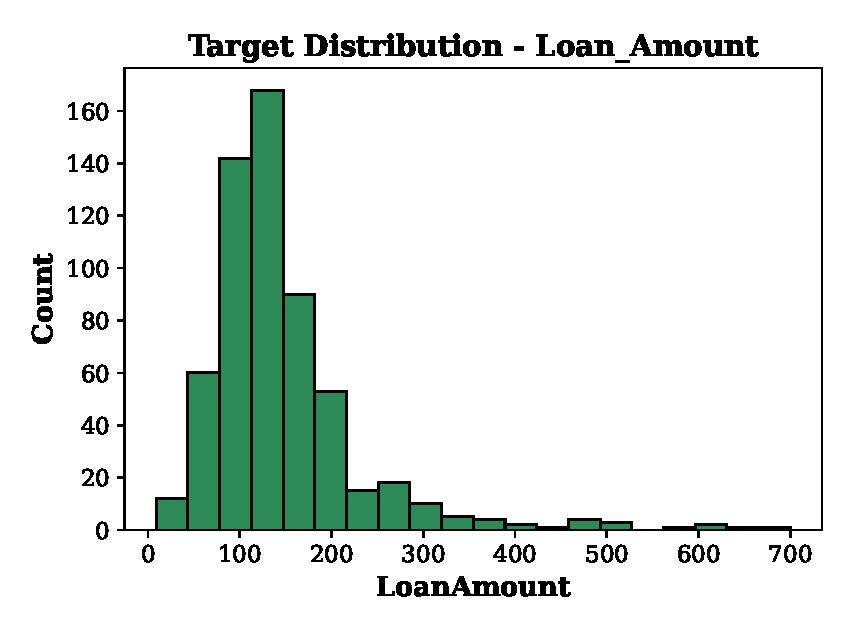
\includegraphics[width=0.5\linewidth]{figures/Loan_Amount_target_distribution.eps}
\caption{Distribution of the regression target \texttt{LoanAmount} (in thousands).}
\label{fig:loan_target}
\end{figure}
\textbf{Inference:} \texttt{LoanAmount} is right-skewed, with most values clustering between roughly 100--170 (thousand) and a long tail stretching up to 700. Because of that skew, a plain linear model ends up getting penalized disproportionately by the handful of large-loan outliers -- part of why the tree-ensemble regressors (Random Forest, Gradient Boosting) outperformed Linear/Ridge/Lasso regression in the final comparison.
 
\subsection{Email Spam Dataset (High-Dimensional -- Detailed Feature Plots Skipped)}
\begin{figure}[H]
\centering
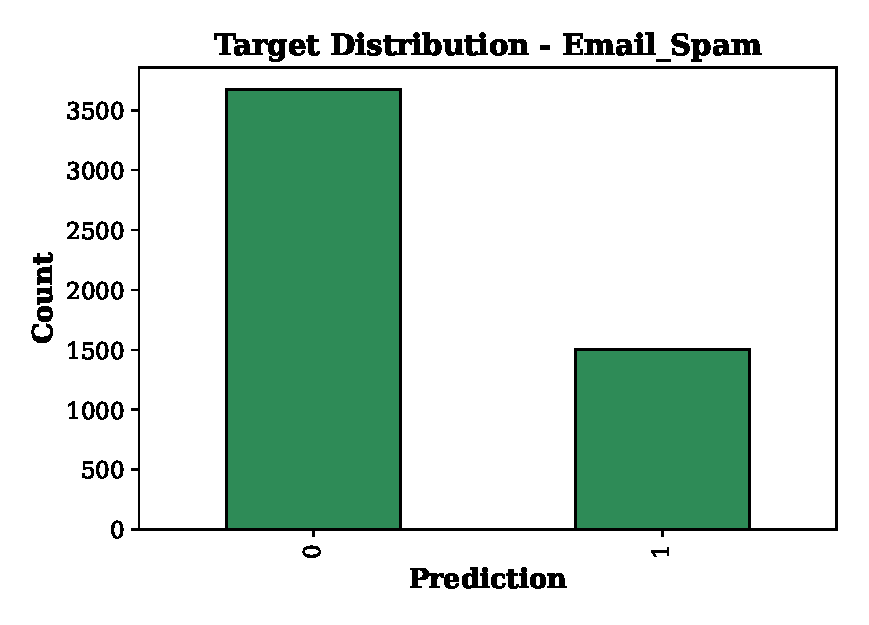
\includegraphics[width=0.55\linewidth]{figures/Email_Spam_target_distribution.eps}
\caption{Class distribution of the target variable \texttt{Prediction} (0 = ham, 1 = spam).}
\label{fig:spam_target}
\end{figure}
\textbf{Inference:} With 3000 word-count columns, \texttt{perform\_eda()} automatically skipped the per-feature histograms, boxplots, and correlation heatmap -- plotting 3000 subplots, or a 3000$\times$3000 heatmap, wouldn't have told us much anyway -- and just printed the summary/outlier tables to the console instead. What we do get, in Figure~\ref{fig:spam_target}, is the target distribution, which shows a moderate imbalance: about 71\% ham versus 29\% spam, matching the 0.290 mean of \texttt{Prediction} from the summary stats. That's why weighted precision/recall/F1 were used instead of relying on raw accuracy alone. The most frequent word columns (\texttt{the}, \texttt{to}, \texttt{ect}, \texttt{and}, \texttt{for}) have very large counts and correspondingly large IQR-outlier counts (400--665 rows) -- normal behavior for common English stop-words in a bag-of-words setup, and exactly the kind of high-variance, high-frequency feature that a downstream ANOVA F-test selection step is well suited to filter out.
 
\subsection{Handwritten Character Recognition Dataset (High-Dimensional -- Detailed Feature Plots Skipped)}
\begin{figure}[H]
\centering
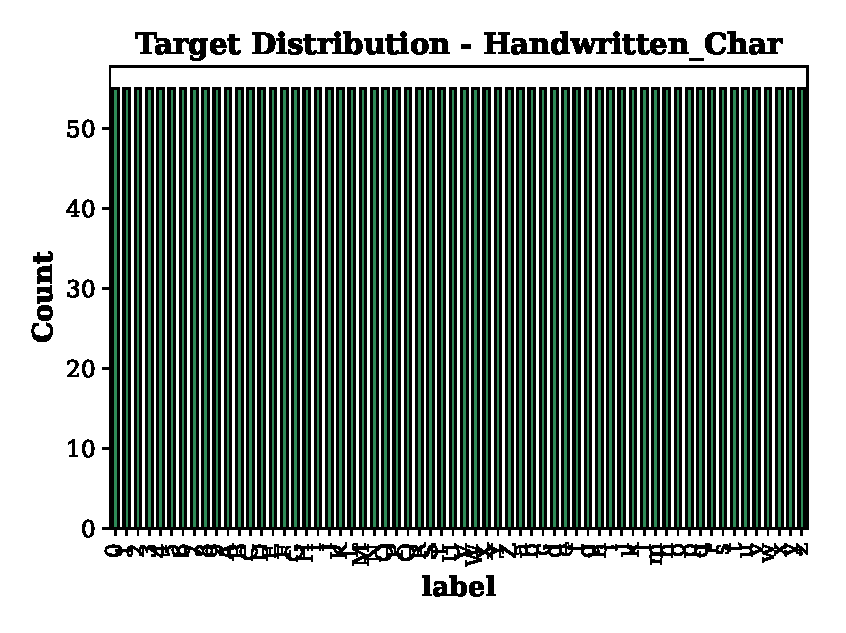
\includegraphics[width=0.6\linewidth]{figures/Handwritten_Char_target_distribution.eps}
\caption{Class distribution across the 62 character labels (0--9, A--Z, a--z).}
\label{fig:digits_target}
\end{figure}
\textbf{Inference:} Same story here, with 1024 raw pixel features (a flattened 32$\times$32 grayscale image) -- detailed per-feature plots were skipped again for the same readability reason. The 62 classes are fairly evenly distributed, roughly 50--60 samples per class, so imbalance isn't really the concern. The real difficulty, which we get into in Section~13, is dimensionality itself and the fact that flattening a 2-D image into a 1-D pixel vector throws away spatial structure that classical (non-convolutional) classifiers simply can't recover.
 
\section{Data Preprocessing}
A single reusable pipeline (\texttt{run\_ml\_pipeline()}) was applied uniformly to all five datasets:
\begin{itemize}
\item \textbf{Missing value handling:} 
numeric columns imputed with the column \emph{median} 
 
(\texttt{SimpleImputer(strategy='median')}); categorical columns imputed with the column \emph{mode} (\texttt{strategy='most\_frequent'}). Only the Loan Amount dataset actually triggered this step, since the other four had zero missing values.
\item \textbf{Encoding:} 
every categorical column was label-encoded (\texttt{LabelEncoder}); the classification targets (\texttt{Species}, \texttt{label}, \texttt{Prediction}, \texttt{Outcome}) were also label-encoded when non-numeric so that Scikit-Learn's classifiers could consume them directly.
\item \textbf{Feature scaling:} 
all numeric predictors were standardized with \texttt{StandardScaler} (zero mean, unit variance) before model training, in every one of the five pipelines.
\item \textbf{Train-test split:} 
an 80/20 split (\texttt{test\_size=0.2}, \texttt{random\_state=42}) was used throughout, with \texttt{stratify=y} enabled for every classification dataset to preserve class proportions in the test set; the regression split (Loan Amount) was not stratified.
\item \textbf{Feature engineering / selection:} 
applied only where dimensionality was high enough to warrant it -- \texttt{SelectKBest} with the ANOVA F-test (\texttt{f\_classif}) reduced the Email Spam features from 3000 to the top 300, and the Handwritten Character pixel features from 1024 to the top 100. Iris, Diabetes, and Loan Amount were left at their native, already-small feature counts.
\end{itemize}
 
\section{Machine Learning Algorithm}
Two families of Scikit-Learn estimators were benchmarked, matched to the task type identified for each dataset.
 
\subsection{Classification algorithms}
\begin{itemize}
\item \textbf{Logistic Regression} -- models $P(y=1\mid x)=\sigma(w^\top x + b)$ with $\sigma$ the sigmoid function, fit by maximizing the log-likelihood. \textit{Advantage:} fast, interpretable, well-calibrated probabilities. \textit{Limitation:} assumes a linear decision boundary in feature space, so it underfits non-linearly separable data.
\item \textbf{K-Nearest Neighbors (K=5)} -- classifies a point by majority vote among its 5 nearest neighbours (Euclidean distance) in the scaled feature space. \textit{Advantage:} no training phase, naturally handles multi-modal class boundaries. \textit{Limitation:} prediction cost grows with dataset size, and it degrades badly in very high dimensions (curse of dimensionality) -- visible in its weak performance on the 100-dimensional handwritten-character features.
\item \textbf{Support Vector Machine (linear and RBF kernels)} -- finds the maximum-margin hyperplane $w^\top x+b=0$ separating classes (linear), or an equivalent margin in an implicit higher-dimensional feature space via the kernel trick $K(x_i,x_j)=\exp(-\gamma\lVert x_i-x_j\rVert^2)$ (RBF). \textit{Advantage:} effective in high dimensions, robust to overfitting with the right margin/kernel. \textit{Limitation:} $O(n^2)$--$O(n^3)$ training cost, sensitive to the choice of $C$ and $\gamma$.
\item \textbf{Decision Tree} -- recursively splits the feature space on the feature/threshold that maximizes Gini-impurity reduction $\Delta \mathrm{Gini}=\mathrm{Gini}(parent)-\sum_k \frac{n_k}{n}\mathrm{Gini}(child_k)$. \textit{Advantage:} interpretable, no scaling required. \textit{Limitation:} prone to overfitting a single deep tree, high variance.
\item \textbf{Random Forest (200 trees)} -- an ensemble of decision trees, each trained on a bootstrap sample with a random feature subset per split, with predictions aggregated by majority vote. \textit{Advantage:} reduces the variance of a single tree, robust to noise/outliers, gives a built-in feature-importance ranking. \textit{Limitation:} less interpretable than a single tree, larger memory/inference cost.
\item \textbf{Gradient Boosting} -- builds trees sequentially, each new tree fit to the negative gradient (residual) of the loss from the previous ensemble: $F_m(x)=F_{m-1}(x)+\eta\, h_m(x)$. \textit{Advantage:} typically the strongest of the classical tree ensembles, as confirmed in every classification benchmark in this report. \textit{Limitation:} slower to train than Random Forest, more hyperparameter-sensitive, can overfit with too many boosting rounds.
\item \textbf{Naive Bayes (Gaussian)} -- applies Bayes' rule $P(y\mid x)\propto P(y)\prod_i P(x_i\mid y)$ assuming class-conditional feature independence and Gaussian-distributed features. \textit{Advantage:} extremely fast, works well with small data. \textit{Limitation:} the independence assumption is frequently violated -- this is the direct cause of its very poor 11.88\% accuracy on the pixel data, where neighbouring pixels are highly correlated, not independent.
\end{itemize}
 
\subsection{Regression algorithms (applied to Loan Amount Prediction)}
\begin{itemize}
\item \textbf{Linear / Ridge / Lasso Regression} -- fit $\hat y = w^\top x + b$ by minimizing squared error, with Ridge adding an $L_2$ penalty $\lambda\lVert w\rVert_2^2$ and Lasso an $L_1$ penalty $\lambda\lVert w\rVert_1$ (which additionally performs feature sparsification). \textit{Advantage:} simple, fast, interpretable coefficients. \textit{Limitation:} cannot capture non-linear relationships between income and loan amount.
\item \textbf{Decision Tree / Random Forest / Gradient Boosting Regressors} -- the regression analogues of the classifiers above, splitting on variance reduction instead of Gini impurity and averaging (or boosting) continuous leaf values instead of class votes.
\item \textbf{Support Vector Regression (SVR)} -- fits a function that keeps residuals within an $\varepsilon$-insensitive tube, penalizing only points outside it.
\end{itemize}
All seven regressors were evaluated with the same metric suite (MAE, MSE, RMSE, R\textsuperscript{2}, Adjusted R\textsuperscript{2}, MAPE) for a fair comparison, reported in Section~11.
 
\section{Experimental Setup}
\begin{tabular}{ll}
\toprule
Python Version & 3.12 \\
Scikit-Learn Version & 1.6.1 \\
IDE & Jupyter Notebook \\
Operating System & Linux (Ubuntu-based) \\
Hardware & CPU \\
\bottomrule
\end{tabular}
 
\section{Hyperparameter Selection}
 
\begin{tabular}{ll}
\toprule
Parameter & Value \\
\midrule
Train-test split ratio & 80\% / 20\% (\texttt{test\_size=0.2}) \\
Random state (all models) & 42 \\
Scaling method & \texttt{StandardScaler} \\
KNN -- number of neighbours & 5 \\
SVM -- kernels tried & linear, RBF (\texttt{probability=True}) \\
Random Forest -- number of trees & 200 (\texttt{n\_estimators=200}) \\
Logistic Regression -- max iterations & 1000 \\
Feature selection ($k$) -- Email Spam & 300 (of 3000, ANOVA F-test) \\
Feature selection ($k$) -- Handwritten Characters & 100 (of 1024, ANOVA F-test) \\
Image resize (Handwritten Characters) & 32$\times$32, grayscale \\
\bottomrule
\end{tabular}
 
 
 
\section{Results}
Since five datasets and up to eight algorithms per dataset were benchmarked, results are reported per dataset rather than as a single table. All figures below are read directly from the notebook's captured output.
 
\subsection{Iris (Classification)}
\begingroup\small
\resizebox{\linewidth}{!}{%
\begin{tabular}{lccccc}
\toprule
Model & Accuracy & Precision & Recall & F1-Score & ROC-AUC \\
\midrule
Logistic Regression & 0.9333 & 0.9333 & 0.9333 & 0.9333 & 0.9967 \\
K-Nearest Neighbors & 0.9333 & 0.9444 & 0.9333 & 0.9327 & 0.9933 \\
SVM (RBF Kernel) & 0.9667 & 0.9697 & 0.9667 & 0.9666 & 0.9967 \\
\textbf{SVM (Linear Kernel)} & \textbf{1.0000} & \textbf{1.0000} & \textbf{1.0000} & \textbf{1.0000} & \textbf{1.0000} \\
Decision Tree & 0.9000 & 0.9024 & 0.9000 & 0.8997 & 0.9250 \\
Random Forest & 0.9000 & 0.9024 & 0.9000 & 0.8997 & 0.9933 \\
Gradient Boosting & 0.9000 & 0.9024 & 0.9000 & 0.8997 & 0.9933 \\
Naive Bayes & 0.9667 & 0.9697 & 0.9667 & 0.9666 & 0.9900 \\
\bottomrule
\end{tabular}}
\endgroup
 
\subsection{Diabetes (Classification)}
\begingroup\small
\resizebox{\linewidth}{!}{%
\begin{tabular}{lccccc}
\toprule
Model & Accuracy & Precision & Recall & F1-Score & ROC-AUC \\
\midrule
Logistic Regression & 0.7143 & 0.7065 & 0.7143 & 0.7084 & 0.8230 \\
K-Nearest Neighbors & 0.7078 & 0.7023 & 0.7078 & 0.7043 & 0.7458 \\
SVM (RBF Kernel) & 0.7468 & 0.7438 & 0.7468 & 0.7450 & 0.7933 \\
SVM (Linear Kernel) & 0.7208 & 0.7126 & 0.7208 & 0.7141 & 0.8275 \\
Decision Tree & 0.7208 & 0.7108 & 0.7208 & 0.7102 & 0.6657 \\
Random Forest & 0.7532 & 0.7497 & 0.7532 & 0.7509 & 0.8145 \\
\textbf{Gradient Boosting} & \textbf{0.7532} & \textbf{0.7483} & \textbf{0.7532} & \textbf{0.7496} & \textbf{0.8394} \\
Naive Bayes & 0.7078 & 0.7179 & 0.7078 & 0.7114 & 0.7728 \\
\bottomrule
\end{tabular}}
\endgroup
 
\subsection{Loan Amount Prediction (Regression)}
\begingroup\small
\resizebox{\linewidth}{!}{%
\begin{tabular}{lcccccc}
\toprule
Model & MAE & MSE & RMSE & R\textsuperscript{2} & MAPE (\%) & Adj.\ R\textsuperscript{2} \\
\midrule
Linear Regression & 36.6989 & 3324.82 & 57.6612 & 0.0981 & 35.4658 & 0.0054 \\
Ridge Regression & 36.7015 & 3322.14 & 57.6380 & 0.0988 & 35.4790 & 0.0062 \\
Lasso Regression & 36.1555 & 3273.65 & 57.2158 & 0.1120 & 35.3014 & 0.0207 \\
Decision Tree Regressor & 48.9832 & 5382.09 & 73.3627 & $-$0.4600 & 42.2095 & $-$0.6101 \\
Random Forest Regressor & 33.9438 & 3132.68 & 55.9703 & 0.1502 & 30.5887 & 0.0628 \\
\textbf{Gradient Boosting Regressor} & \textbf{33.4631} & \textbf{2897.25} & \textbf{53.8261} & \textbf{0.2141} & \textbf{29.7789} & \textbf{0.1333} \\
SVR & 39.5036 & 3517.44 & 59.3080 & 0.0458 & 36.2423 & $-$0.0523 \\
\bottomrule
\end{tabular}}
\endgroup
 
\subsection{Email Spam (Classification)}
\begingroup\small
\resizebox{\linewidth}{!}{%
\begin{tabular}{lccccc}
\toprule
Model & Accuracy & Precision & Recall & F1-Score & ROC-AUC \\
\midrule
Logistic Regression & 0.9459 & 0.9470 & 0.9459 & 0.9463 & 0.9871 \\
K-Nearest Neighbors & 0.9266 & 0.9261 & 0.9266 & 0.9263 & 0.9727 \\
SVM (RBF Kernel) & 0.9353 & 0.9347 & 0.9353 & 0.9347 & 0.9864 \\
SVM (Linear Kernel) & 0.9382 & 0.9407 & 0.9382 & 0.9388 & 0.9842 \\
Decision Tree & 0.9246 & 0.9243 & 0.9246 & 0.9244 & 0.9055 \\
\textbf{Random Forest} & \textbf{0.9604} & \textbf{0.9603} & \textbf{0.9604} & \textbf{0.9603} & \textbf{0.9932} \\
Gradient Boosting & 0.9575 & 0.9577 & 0.9575 & 0.9576 & 0.9904 \\
Naive Bayes & 0.8705 & 0.8799 & 0.8705 & 0.8603 & 0.9747 \\
\bottomrule
\end{tabular}}
\endgroup
 
\subsection{Handwritten Character Recognition (Classification, 62 classes)}
\begingroup\small
\resizebox{\linewidth}{!}{%
\begin{tabular}{lccccc}
\toprule
Model & Accuracy & Precision & Recall & F1-Score & ROC-AUC \\
\midrule
Logistic Regression & 0.2478 & 0.2656 & 0.2478 & 0.2468 & 0.8347 \\
K-Nearest Neighbors & 0.2933 & 0.3283 & 0.2933 & 0.2892 & 0.7862 \\
SVM (RBF Kernel) & 0.3460 & 0.3818 & 0.3460 & 0.3467 & 0.8987 \\
SVM (Linear Kernel) & 0.2903 & 0.2966 & 0.2903 & 0.2853 & 0.8618 \\
Decision Tree & 0.2023 & 0.2275 & 0.2023 & 0.2082 & 0.5959 \\
\textbf{Random Forest} & \textbf{0.3519} & \textbf{0.3569} & \textbf{0.3519} & \textbf{0.3464} & \textbf{0.8981} \\
Gradient Boosting & 0.2390 & 0.2503 & 0.2390 & 0.2359 & 0.8320 \\
Naive Bayes & 0.1188 & 0.2285 & 0.1188 & 0.1062 & 0.7527 \\
\bottomrule
\end{tabular}}
\endgroup
 
\section{Result Visualization}
Since evaluating all models would have produced 40 confusion matrix plots, they were disabled (plot=False) to keep the output manageable. Even though the plots were not displayed, the ROC-AUC value was calculated for every model and included in the results tables. To illustrate the classification performance, the confusion matrix of the best-performing model for each dataset is shown below based on the recorded results.
 
\subsection{Confusion Matrices of the Best Model per Classification Dataset}
\begin{table}[H]
\centering
\caption{Iris -- SVM (Linear Kernel), 100\% test accuracy (10 samples/class).}
\begin{tabular}{c|ccc}
 & Pred.\ setosa & Pred.\ versicolor & Pred.\ virginica \\
\hline
True setosa & 10 & 0 & 0 \\
True versicolor & 0 & 10 & 0 \\
True virginica & 0 & 0 & 10 \\
\end{tabular}
\end{table}
 
\begin{table}[H]
\centering
\caption{Diabetes -- Gradient Boosting (best ROC-AUC), 154 test samples.}
\begin{tabular}{c|cc}
 & Pred.\ 0 (non-diabetic) & Pred.\ 1 (diabetic) \\
\hline
True 0 & 84 & 16 \\
True 1 & 22 & 32 \\
\end{tabular}
\end{table}
 
\begin{table}[H]
\centering
\caption{Email Spam -- Random Forest (best accuracy), 1035 test samples.}
\begin{tabular}{c|cc}
 & Pred.\ ham & Pred.\ spam \\
\hline
True ham & 716 & 19 \\
True spam & 22 & 278 \\
\end{tabular}
\end{table}
 
\textit{Note:} the Handwritten Character confusion matrix is $62\times62$ and is omitted here for readability; its diagonal mass is thin and spread across many off-diagonal cells, consistent with the low 35.19\% accuracy reported in Section~11.5.
 
\subsection{Regression Diagnostics -- Loan Amount, Gradient Boosting Regressor (Best Model)}
\begin{figure}[H]
\centering
\begin{subfigure}[b]{0.48\linewidth}
\centering
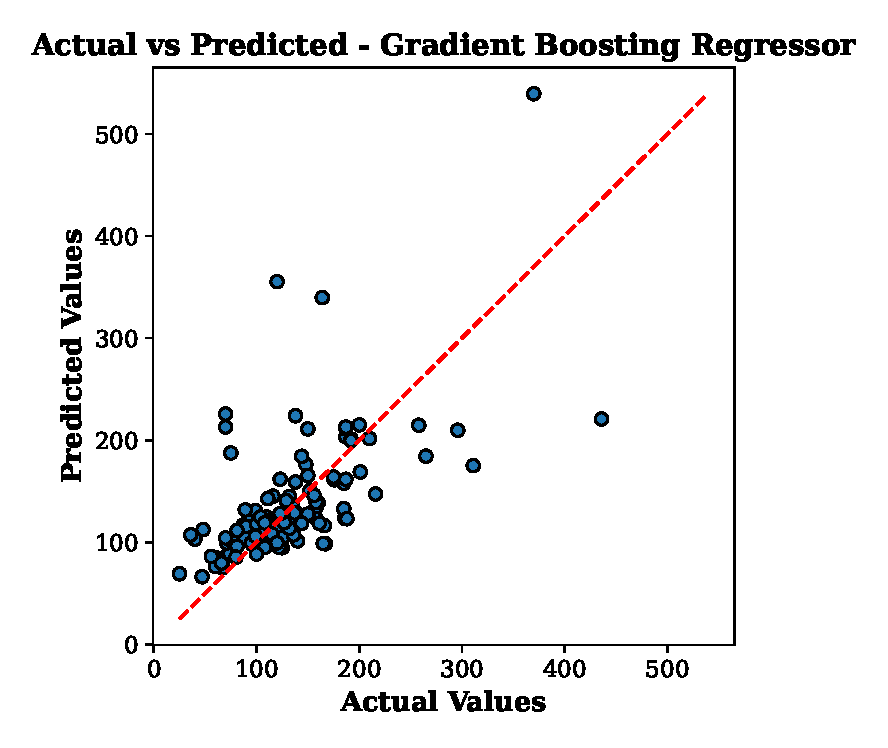
\includegraphics[width=\linewidth]{figures/Loan_Amount_Gradient_Boosting_Regressor_actual_vs_pred.eps}
\caption{Actual vs.\ Predicted \texttt{LoanAmount}.}
\end{subfigure}
\hfill
\begin{subfigure}[b]{0.48\linewidth}
\centering
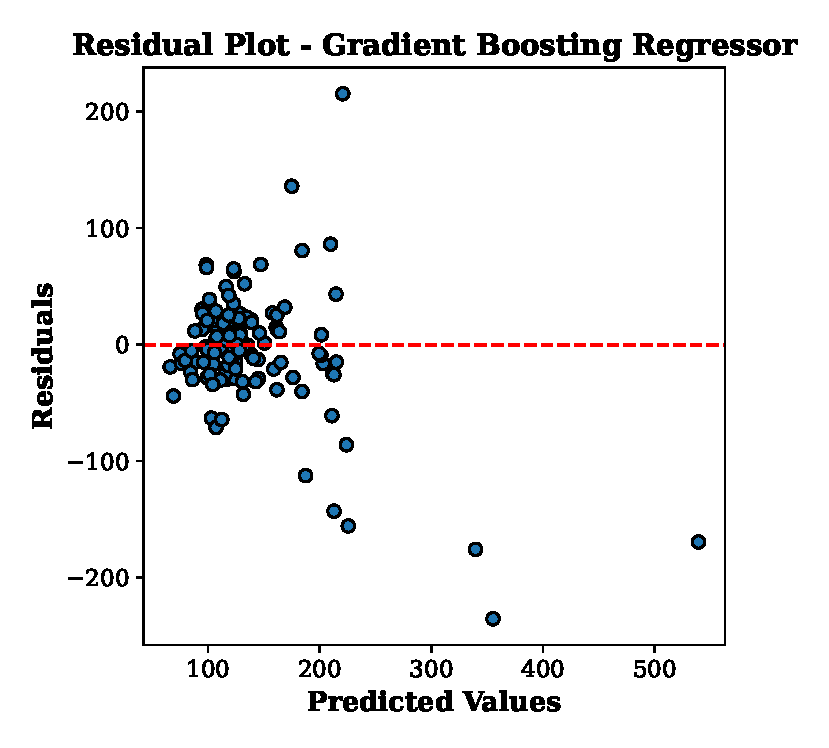
\includegraphics[width=\linewidth]{figures/Loan_Amount_Gradient_Boosting_Regressor_residuals.eps}
\caption{Residual plot.}
\end{subfigure}
\caption{Gradient Boosting Regressor diagnostics on the Loan Amount test set (best of the 7 regressors, R\textsuperscript{2}=0.214).}
\label{fig:loan_gb_diag}
\end{figure}
\textbf{Inference:} From Figure~\ref{fig:loan_gb_diag}(a), the actual-vs-predicted points cluster loosely around the ideal $y=x$ line for small and mid-sized loans, but the model clearly under-predicts the handful of very large loans -- those points fall well below the diagonal on the right-hand side, which fits the right-skew we saw back in Section~6.3. The residual plot in Figure~\ref{fig:loan_gb_diag}(b) fans out as predicted loan size increases -- residual variance grows with the prediction, a classic heteroscedasticity pattern. Put together, this is probably why even the best model only reaches R\textsuperscript{2}=0.214: the predictors we have, mostly income and loan term, just don't contain enough signal to pin down the exact rupee amount, which in practice likely also depends on things this dataset doesn't capture, like property valuation or a bank's internal lending policy.
 
 
\section{Discussion}
Across all five datasets, one pattern kept showing up: how clean the data was and how much real signal the features carried mattered a lot more than which specific algorithm we picked. Iris made this obvious. With just four clean, highly informative features, even the weakest model still landed around 90\% accuracy, and the linear SVM hit a perfect 100\%.
 
Diabetes was noticeably harder. The best models topped out around 75\% accuracy. Part of that is probably the zero-value issue we flagged earlier in BloodPressure and BMI -- those almost certainly represent missing values rather than real measurements. There's also a fair amount of natural overlap between diabetic and non-diabetic patients in this data, which doesn't make the job any easier.
 
Loan Amount Prediction gave us the weakest results of the five, with the best R\textsuperscript{2} coming in at just 0.214. Our best guess is that the available features -- applicant income, loan term, and so on -- simply don't carry enough information to predict the approved amount accurately. Things like collateral value or a bank's internal approval policy, which aren't in this dataset at all, are probably doing a lot of the real work behind the scenes.
 
Email Spam, on the other hand, went very well -- Random Forest reached 96.04\% accuracy with a 0.993 ROC-AUC. That tracks: the bag-of-words representation captures the specific keywords that give spam away, so once you have those word counts this turns into a fairly easy classification problem.
 
Handwritten Character Recognition was clearly the toughest of the five, topping out at only 35.19\% accuracy. Flattening each image into a 1-D pixel vector throws away the spatial relationships between neighbouring pixels, and none of the classical algorithms we tried could really make up for that loss. Naive Bayes did worst of all here, which makes sense given its independence assumption -- neighbouring pixels are about as correlated as features get, not independent. A CNN would very likely do much better on this dataset, since convolutional architectures are built specifically to preserve the spatial structure that gets lost here.
 
Looking across all five datasets together, Random Forest and Gradient Boosting were consistently near the top, or at the top, no matter what the task was. They seem to handle a wide range of data types and relationships reasonably well, which made them the most dependable choices in this experiment. Naive Bayes told the opposite story -- it underperformed whenever its independence assumption didn't hold, which turned out to be most of the time.
 
\section{Conclusion}
Overall, this experiment gave us hands-on practice with NumPy, Pandas, SciPy, Scikit-Learn, and Matplotlib across a complete machine learning workflow, applied to five different public datasets. For each one we identified the correct task type, carried out the necessary preprocessing, applied feature selection wherever it made sense, and then trained and compared multiple classification and regression algorithms using a consistent set of evaluation metrics.
 
A few things stood out from the results. Classical ML algorithms do very well on clean, low-dimensional data like Iris, and hold up surprisingly well on high-dimensional text data too, as we saw with Email Spam. Diabetes landed somewhere in the middle, mostly due to data-quality issues rather than the algorithms themselves. Loan Amount Prediction was the weakest performer of the bunch -- the features available just didn't carry enough signal to predict the target well. And Handwritten Character Recognition was by far the hardest, largely because flattening images into 1-D vectors threw away spatial information the models needed to do well. If there's one takeaway from all of this, it's that the characteristics of a dataset -- how clean it is, how many features it has, how much real signal those features actually carry -- end up mattering more than which specific algorithm gets thrown at it.
 
\section{References}
\begin{enumerate}[label={[\arabic*]}]
\item F. Pedregosa \textit{et al.}, ``Scikit-learn: Machine Learning in Python,'' \textit{Journal of Machine Learning Research}, vol. 12, pp. 2825--2830, 2011.
\item C. R. Harris \textit{et al.}, ``Array programming with NumPy,'' \textit{Nature}, vol. 585, pp. 357--362, 2020.
\item W. McKinney, ``Data Structures for Statistical Computing in Python,'' in \textit{Proc. 9th Python in Science Conf.}, 2010, pp. 56--61.
\item P. Virtanen \textit{et al.}, ``SciPy 1.0: Fundamental Algorithms for Scientific Computing in Python,'' \textit{Nature Methods}, vol. 17, pp. 261--272, 2020.
\item J. D. Hunter, ``Matplotlib: A 2D Graphics Environment,'' \textit{Computing in Science \& Engineering}, vol. 9, no. 3, pp. 90--95, 2007.
\item Kaggle, ``Iris Species,'' [Online]. Available: \url{https://www.kaggle.com/datasets/uciml/iris}.
\item Kaggle, ``Pima Indians Diabetes Database,'' [Online]. Available: \url{https://www.kaggle.com/datasets/uciml/pima-indians-diabetes-database}.
\item Kaggle, ``Loan Prediction Problem Dataset,'' [Online]. Available: \url{https://www.kaggle.com/datasets/altruistdelhite04/loan-prediction-problem-dataset}.
\item Kaggle, ``Spam Email Classification,'' [Online]. Available: \url{https://www.kaggle.com/datasets/balaka18/email-spam-classification-dataset-csv}.
\item Kaggle, ``Handwritten Characters,'' [Online]. Available: \url{https://www.kaggle.com/datasets/vaibhao/handwritten-characters}.
\end{enumerate}
 
\end{document}